
\section{Idea}
That is, the computation complexity of k-SNFT problem is NP, how do we propose reasonable heuristic methods to solve the problem? Moreover, existed optimal algorithms is all exponential time algorithm.


For example, we suppose a general graph as show in Fig.\ref{fig:DecomposeGraph_orginalgraph}, which consist of tree, path and biconnected component, therefore requesting the k-SNFT graph of the original graph is intractable. That is, we firstly utilized biconnected component algorithm to partition the original graph into two styles of graph(tree graph and biconnected component graph. Besides, small granularity's graphs is easily to be dealed and calculated as show in fig.\ref{fig:DecomposeGraph_elementarygraph}, however the original problem of k-SNFT is reduced into approximated optimal answer problem. Then we obtain any node fault-tolerant graph with service functions of every graphs of small granularity. At last, we integrate all 1-SNFT graphs of small granularity into the final 1-SNFT graph original graph. The advantages of our heuristic method are minimizing the effort required for reconfiguration and parallelly processing every graphs of small granularity which is easily to be solved.

\subsection{Non-optimal to Redundant Links Without swapping}
To overcome the aforementioned limitations and time complexity\ref{sec:Complexity}, we choose decompose original general graph into elementary graphs of small granularity, at the expense of incurring more redundant resources for non-optimal solution but time-efficient. Adding link to elementary graph is much more stable for whole virtual network and reduce swapping/rearrangement problem of whole graph.

\begin{figure}
\centering
% Requires \usepackage{graphicx}
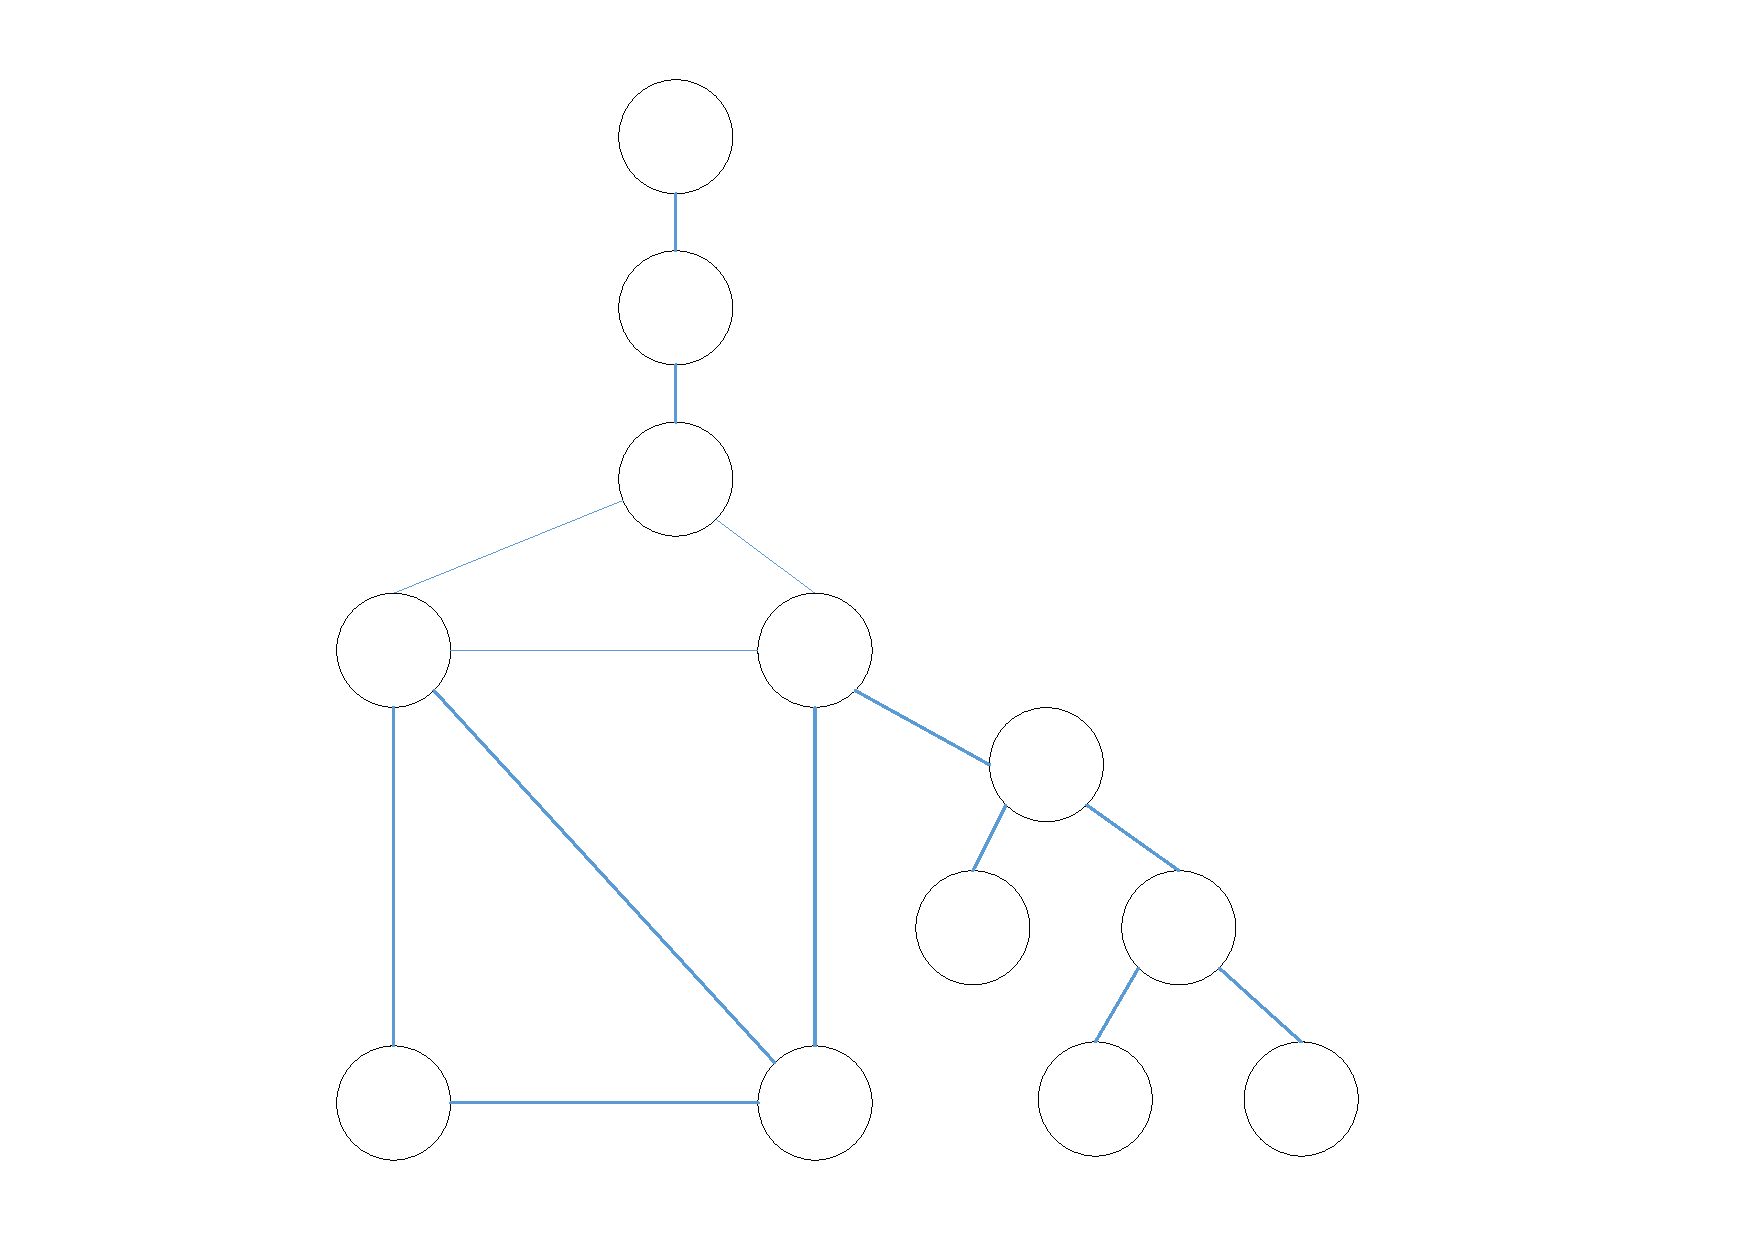
\includegraphics[width=1.5in]{Fig/DecomposeGraph_orginalgraph}\\
\caption{General Graph}\label{fig:DecomposeGraph_orginalgraph}
\end{figure}
\begin{figure}
\centering
% Requires \usepackage{graphicx}
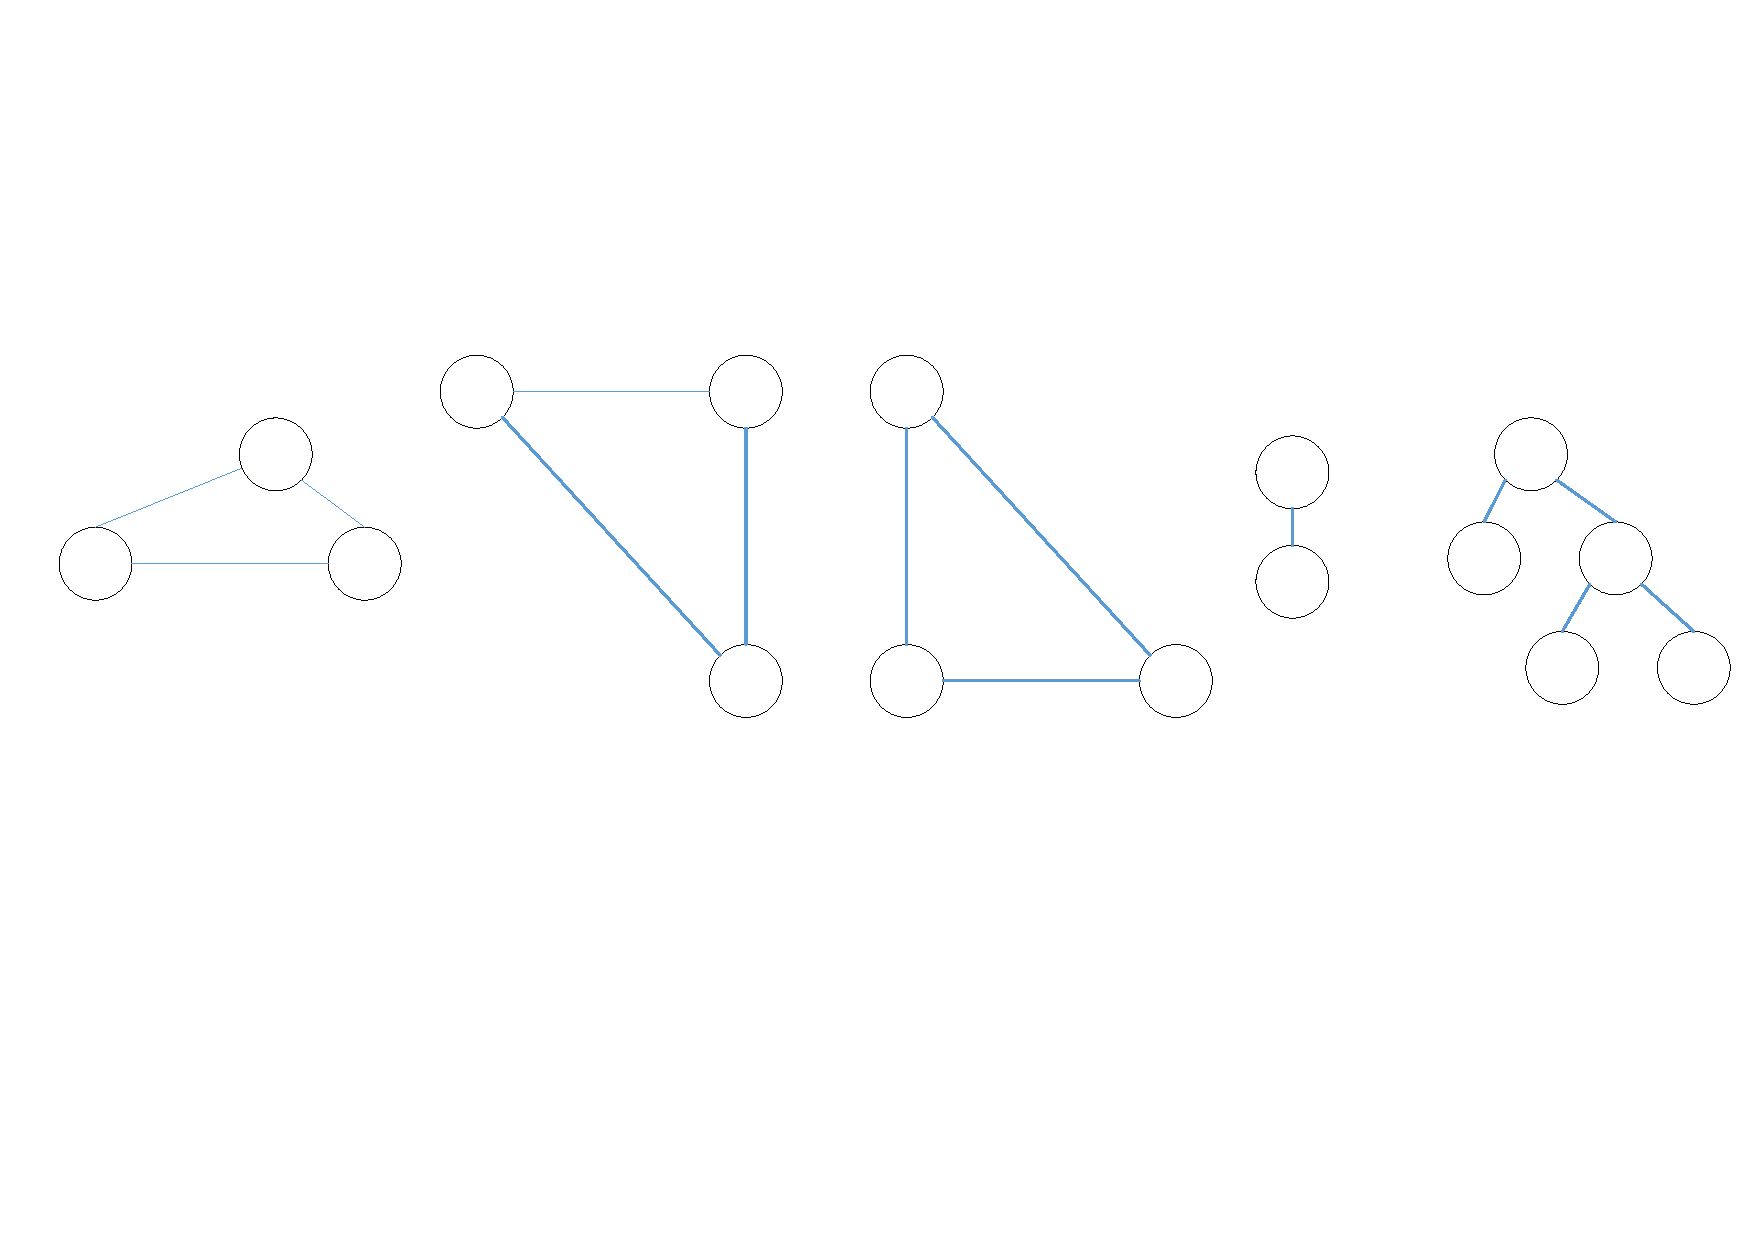
\includegraphics[width=1.5in]{Fig/DecomposeGraph_elementarygraph}\\
\caption{Elementary Graph}\label{fig:DecomposeGraph_elementarygraph}
\end{figure}
\begin{figure}
\centering
% Requires \usepackage{graphicx}
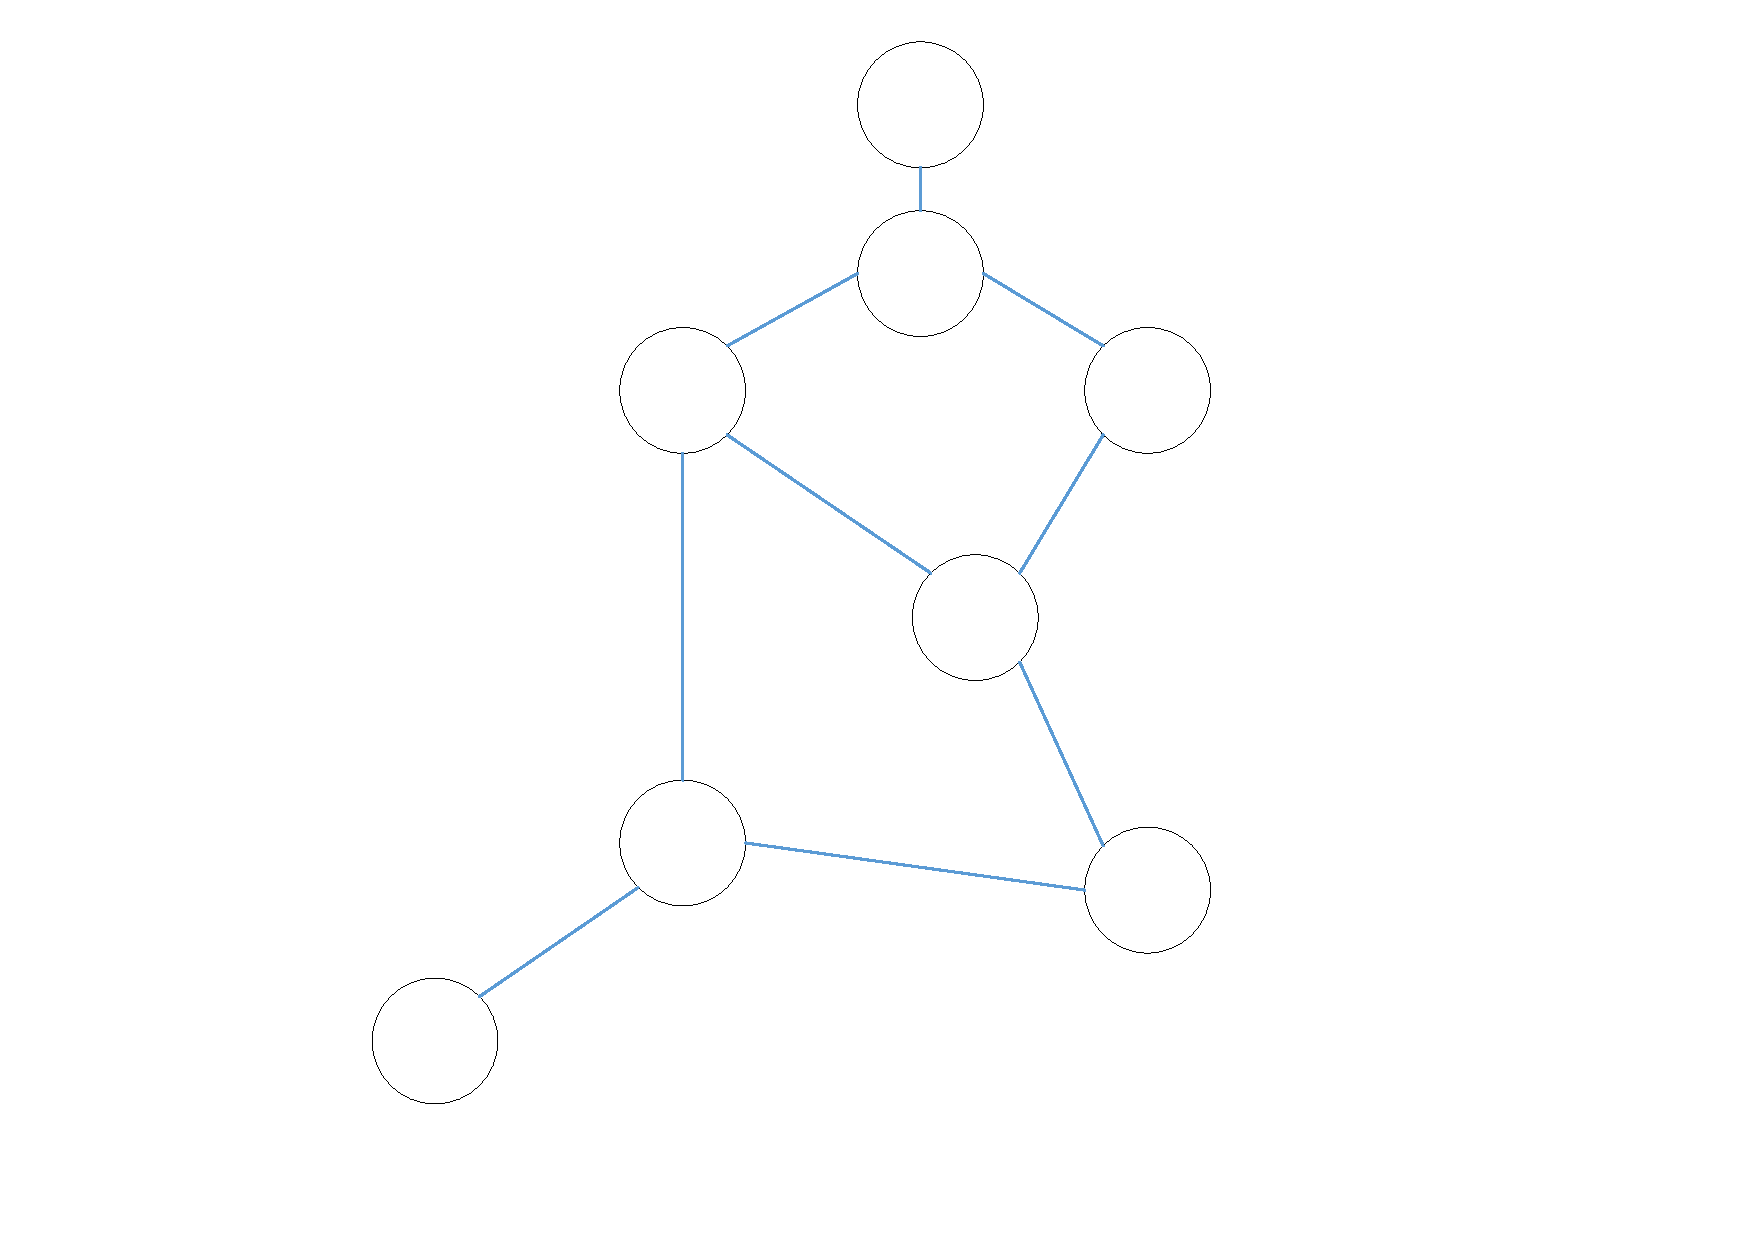
\includegraphics[width=1.5in]{Fig/DecomposeGraph_addnode4mimicycle}\\
  \caption{add node for request minimum cycle of biconnected component graph from Decomposition of Originnal Graph}\label{fig:DecomposeGraph_addnode4mimicycle}
\end{figure}
\begin{figure}
\centering
% Requires \usepackage{graphicx}
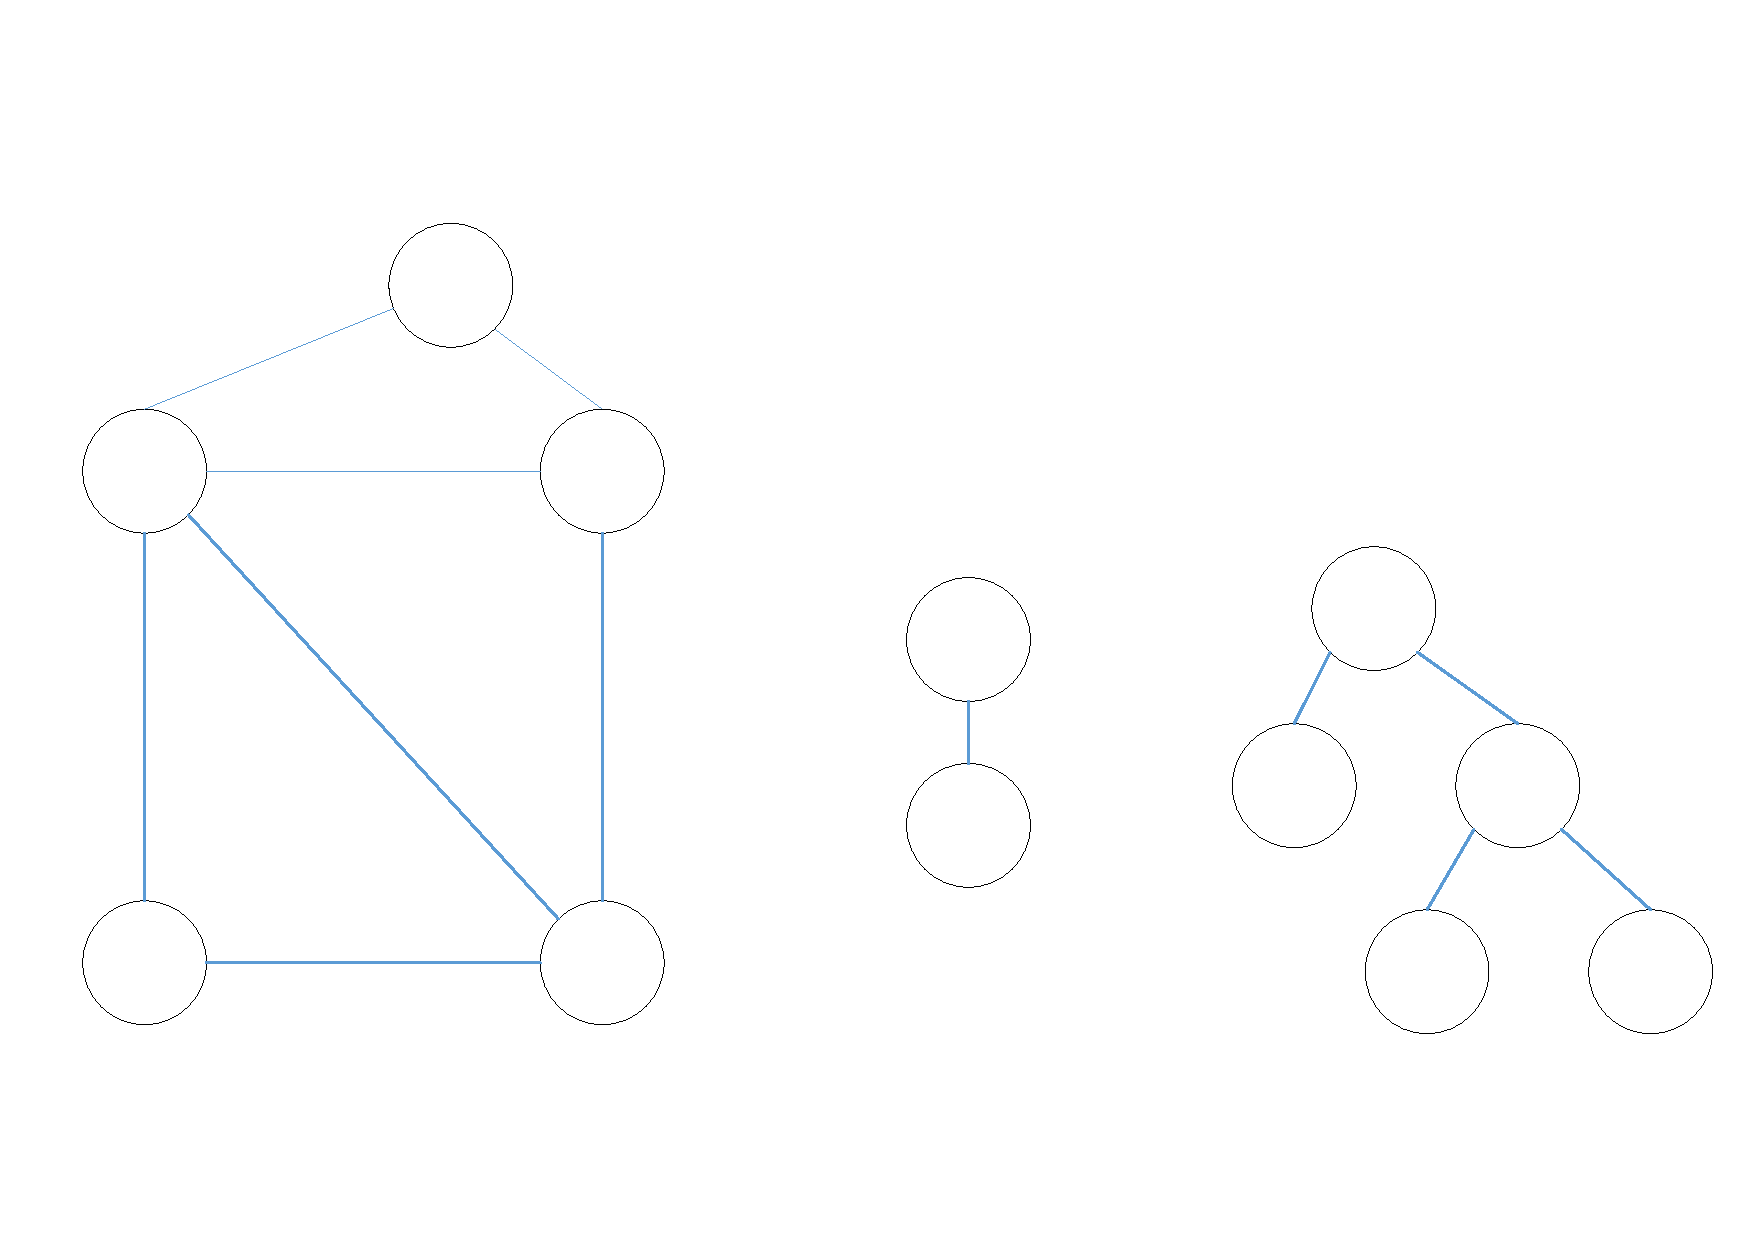
\includegraphics[width=1.5in]{Fig/DecomposeGraph_subbiconnectedgraph}\\
\caption{BCC or non-BCC($subG_i$)}\label{fig:DecomposeGraph_subbiconnectedgraph}
\end{figure}

